\section{Summary}

\begin{frame}{web security summary (1)}
    \begin{itemize}
    \item browser as OS:
        \begin{itemize}
        \item websites are like programs
        \end{itemize}
    \item cross-site scripting
        \begin{itemize}
        \item command injection for the web
        \item not just stuff to display --- program code for website
        \item problem: runs with website permissions (e.g. cookies)
        \end{itemize}
    \end{itemize}
\end{frame}

\begin{frame}{web security summary (2)}
    \begin{itemize}
    \item isolation mechanism: same origin policy
        \begin{itemize}
        \item decision: everything on domain name is ``the same''
        \end{itemize}
    \item cross-site request forgery
        \begin{itemize}
        \item consequence of statelessness
        \item \myemph{all requests} send cookie (password-equivalent)
        \item extra token to distinguish ``user initiated'' or not
        \end{itemize}
    \end{itemize}
\end{frame}

\section{User Tracking}

\begin{frame}{on user tracking}
    \begin{itemize}
    \item embedding one web page in another enables tracking users across website
    \item example: multiple webpages include \texttt{iframe} with a google ad
        \begin{itemize}
        \item your browser sends request \myemph{to Google with same cookie}
        \item Google reliably gets excerpt of web history
        \end{itemize}
    \item reason: websites cooperated with Google
    \item users often don't like this
    \item what can browsers do about this?
    \end{itemize}
\end{frame}

\begin{frame}{changing the cookie policy (1)}
    \begin{itemize}
    \item idea: no ``third-party'' cookies
    \item only send cookies for URL in address bar
    \vspace{.5cm}
    \item<2> now embedded Google calendar can't use my credentials
    \item<2> what about websites that use multiple domains?
    \end{itemize}
\end{frame}

\begin{frame}{changing the cookie policy (2)}
    \begin{itemize}
    \item by default: don't send cookies on embedded cross-origin requests
    \item varying ideas about restricting third-party cookies
    \end{itemize}
\end{frame}

\begin{frame}{third-party cookie restrictions}
    \begin{itemize}
    \item Firefox:
        \begin{itemize}
        \item separate `cookie jar' for each top-level domain
        \item tracker.com loaded from foo.com != tracker.com loaded from bar.com
        \item \myemph<2>{heuristics to avoid breaking some websites}
        \end{itemize}
    \item Safari
        \begin{itemize}
        \item don't see third-party cookies
        \item opt-in to separate cookie jar?
        \end{itemize}
    \item Chrome:
        \begin{itemize}
        \item opt-in to partitioned cookie jar
        \end{itemize}
    \end{itemize}
\end{frame}

% FIXME: heuristics


\begin{frame}[fragile,label=noCookieTrack]{tracking without cookies}
    \begin{itemize}
    \item websites can do tracking even with no cookies
        \begin{itemize}
        \item information in URLs --- add \texttt{?sessionID} to all links
        \item web page caches
        \end{itemize}
    \item websites can ``fingerprint'' browser and machine
        \begin{itemize}
        \item version, fonts, screen resolution, plugins, graphics features, \ldots
        \item \myemph<2>{caching} of previously downloaded resources
        \item almost unique a surprising amount of the time
        \end{itemize}
    \item have IP addresses, too --- very good hints
    \end{itemize}
\end{frame}

\section{Web Frameworks}

\begin{frame}[fragile,label=webFramework]{Web Frameworks}
    \begin{itemize}
    \item tools for making writing interactive websites help
    \item e.g. Django (Python): 
        \begin{itemize}
            \item default to anti-embedding HTTP header (no clickjacking)
        \item default to HttpOnly cookies
        \item default to requiring CSRF token for POSTs
        \end{itemize}
    \item usually provide ``templates'' which escape HTML properly by default
        \begin{itemize}
            \item template: \verb|<p>Name: {{name}}| (placeholder in \{\{\ldots\}\})
            \item if name is \verb|<script>...| result is \verb|<p>Name: &lt;script&gt;...|
        \end{itemize}
    \end{itemize}
\end{frame}
% FIXME:

\section{client security}

\begin{frame}[fragile,label=UAFTriggering]{recall: UAF triggering code}
    \begin{itemize}
    \item earlier in semester: exploit in Chrome \myemph{browser} itself
    \end{itemize}
\lstset{
    language=JavaScript,
    style=smaller,
    moredelim={**[is][\btHL<2|handout:0>]{~2~}{~end~}},
    moredelim={**[is][\btHL<3-4|handout:0>]{~3~}{~end~}},
    moredelim={**[is][\btHL<4|handout:0>]{~4~}{~end~}},
}
\begin{tikzpicture}
\node[anchor=north east] (code) at (0, 0) {
\begin{lstlisting}
// in HTML near this JavaScript:
// <video id="vid"> (video player element)
function source_opened() {
  buffer = ms.addSourceBuffer('video/webm; codecs="vorbis,vp8"');
  ~2~vid.parentNode.removeChild(vid);~end~
  gc(); // force garbage collector to run now
  // garbage collector frees unreachable objects
  // (would be run automatically, eventually, too)
  // buffer now internally refers to delete'd player object
  ~3~buffer.timestampOffset = 42;~end~
}
ms = new WebKitMediaSource();
ms.addEventListener('webkitsourceopen', source_opened);
vid.src = window.URL.createObjectURL(ms);
\end{lstlisting}
};
\end{tikzpicture}
\end{frame}

\begin{frame}{browsers and exploits}
    \begin{itemize}
    \item browsers are in a particularly dangerous position for exploits
    \item \myemph{routinely run untrusted code} (JavaScript on websites)
    \item huge amounts of code, often written in C/C++
        \begin{itemize}
            \item WebKit (part of Chrome, Safari) has millions of lines of code
        \end{itemize}
    \end{itemize}
\end{frame}

\begin{frame}{malvertising}
    \begin{itemize}
    \item could trick user into visiting your website
        \vspace{.5cm}
    \item or pay for ad --- embed your webpage in another!
        \begin{itemize}
        \item can run whatever script you like
        \end{itemize}
    \end{itemize}
    %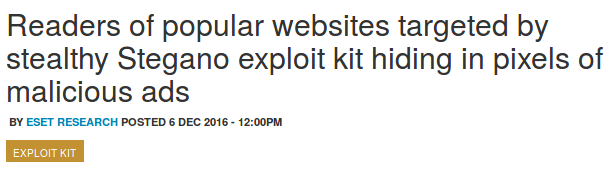
\includegraphics[width=0.9\textwidth]{malvert-stegano} % FIXME
\end{frame}

\begin{frame}{modern advertising landscape (1)}
    \begin{itemize}
        \item website ads are often \myemph{sold in realtime}
        \item conceptual idea: \myemph{mini-auction} for every ad
        \item major concerns about fraud
            \begin{itemize}
            \item are you really showing my ad?
            \end{itemize}
        \item ad operators want to do own tracking
            \begin{itemize}
            \item get better idea what to show/bid
            \end{itemize}
    \end{itemize}
\end{frame}

\begin{frame}{modern advertising landscape (2)}
    \begin{itemize}
        \item website operators \myemph{typically don't host ads}
            \begin{itemize}
            \item don't build own realtime auction infrastructure
            \item not trusted to report number of ad views correctly
            \end{itemize}
        \item ads often sold indirectly
            \begin{itemize}
            \item middleman handles bidding/etc.
            \item website operators sell to multiple ad operators
            \end{itemize}
    \end{itemize}
\end{frame}



